\section{An\'alisis}
Este prototipo determina una clasificaci\'on de las conversaciones en 4 niveles de peligrosidad: No peligrosa, Poco peligrosa, Peligrosa y Muy peligrosa. 

\subsection{Objetivo}
Ralizar un m\'odulo que sea capaz de determinar el nivel de peligrosidad de una conversaci\'on en las siguientes clases: No peligrosa, Poco peligrosa, Peligrosa y Muy peligrosa. 

\subsection{Caracter\'isticas}
\begin{description}
\item[FEAT1:] El sistema analiza el vector generado en el prototipo 2.
\item[FEAT2:] El sistema toma como entrada la clase resultante del prototipo 3.
\item[FEAT3:] Se plantea un modelo mediante una red neuronal para la clasificaci\'on.

\end{description}

\subsection{Restricciones}

\begin{itemize}
\item  Uso de t\'ecnicas de l\'ogica difusa.
\item  Prototipo programado en Octave versi\'on 3.8.
\end{itemize}

\subsection{Marco Te\'orico}
\subsubsection{Red Neuronal}
Las redes neuronales son sistemas ideados como abstracciones de las estructuras neurobiol\'ogicas encontradas en la naturaleza y tienen la caracter\'istica de ser sistemas desordenados capaces de guardar informaci\'on.

La forma en que desarrollan su trabajo es esencialmente distinta de la utilizada por las computadoras convencionales. Los procesadores microsc\'opicos del cerebro (neuronas) operan en paralelo y presentan cualitativamente m\'as ruido que los elementos que forman a las computadoras. No ejecutan un programa fijo con base en un conjunto previamente especificado de datos, sino que comunican se\~nales a trav\'es de retransmisores que llamamos sin\'apsis, que llegan a centros de conjunci\'on llamados los cuerpos de las neuronas y desde los cuales surgen señales el\'ectricas a trav\'es de canales conocidos con el nombre de axones.

La importancia de cada sin\'apsis en el proceso de retransmisi\'on se actualiza continuamente y lo mismo ocurre con algunas propiedades intr\'insecas de las neuronas, proporcionando un sistema de autoprogramaci\'on y adaptaci\'on que sustituye a la programaci\'on externa de los sistemas de c\'omputo comunes. Existe as\'i una din\'amica de las sin\'apsis y de las neuronas en el cual los programas y los datos cambian todo el tiempo.

\subsubsection{BackPropagation}

La propagaci\'on hacia atr\'as de errores o retropropagaci\'on (del ingl\'es backpropagation) es un algoritmo de aprendizaje supervisado que se usa para entrenar redes neuronales artificiales. El algoritmo emplea un ciclo propagaci\'on – adaptaci\'on de dos fases. Una vez que se ha aplicado un patr\'on a la entrada de la red como est\'imulo, este se propaga desde la primera capa a trav\'es de las capas superiores de la red, hasta generar una salida. 

\subsubsection{L\'ogica difusa}
La l\'ogica difusa es una extensi\'on de la l\'ogica tradicional(Booleana) que utiliza conceptos de pertenencia de sistemas parecidos a la manera de pensar humana.

A partir de la  observaci\'on del nivel 3 de la matriz de caracterizaci\'on se hace notar, este nivel, como discriminante para diferenciar una conversaci\'on peligrosa de otra no peligrosa a partir de la media. Se obtuvo una media 3 incidencias de ese nivel en conversaciones peligrosas. De acuerdo a esto se dedujo la tabla \ref{tab:TablaNiveles}.



\begin{longtable}{|c|c|c|c|c|c|c|c|c|c|c|}

\hline
N1 & N2 & N3 & N3\_2 & N4 & N5 & N6 & No Peligrosa & Poco Peligrosa & Peligrosa & Muy Peligrosa \\
\hline
\endfirsthead


\hline
N1 & N2 & N3 & N3\_2 &  N4 & N5 & N6 & No Peligrosa & Poco Peligrosa & Peligrosa & Muy Peligrosa \\
\hline
\endhead
\hline
\multicolumn{11}{c}{Sigue en la p\'agina siguiente.}
\endfoot
\endlastfoot


0 & 0 & 0 & 0 & 0 & 0 & 0 &  1 & 0 & 0 & 0 \\
0 & 0 & 0 & 0 & 0 & 0 & 1 &  0 & 1 & 0 & 0 \\
0 & 0 & 0 & 0 & 0 & 1 & 0 &  0 & 0 & 0 & 1 \\
0 & 0 & 0 & 0 & 0 & 1 & 1 &  0 & 0 & 0 & 1 \\
0 & 0 & 0 & 0 & 1 & 0 & 0 &  0 & 0 & 1 & 0 \\
0 & 0 & 0 & 0 & 1 & 0 & 1 &  0 & 0 & 1 & 0 \\
0 & 0 & 0 & 0 & 1 & 1 & 0 &  0 & 0 & 0 & 1 \\
0 & 0 & 0 & 0 & 1 & 1 & 1 &  0 & 0 & 0 & 1 \\
0 & 0 & 0 & 1 & 0 & 0 & 0 &  0 & 1 & 0 & 0 \\
0 & 0 & 0 & 1 & 0 & 0 & 1 &  0 & 0 & 1 & 0 \\
0 & 0 & 0 & 1 & 0 & 1 & 0 &  0 & 0 & 0 & 1 \\
0 & 0 & 0 & 1 & 0 & 1 & 1 &  0 & 0 & 0 & 1 \\
0 & 0 & 0 & 1 & 1 & 0 & 0 &  0 & 0 & 1 & 0 \\
0 & 0 & 0 & 1 & 1 & 0 & 1 &  0 & 0 & 1 & 0 \\
0 & 0 & 0 & 1 & 1 & 1 & 0 &  0 & 0 & 0 & 1 \\
0 & 0 & 0 & 1 & 1 & 1 & 1 &  0 & 0 & 0 & 1 \\
0 & 0 & 1 & 0 & 0 & 0 & 0 &  1 & 0 & 0 & 0 \\
0 & 0 & 1 & 0 & 0 & 0 & 1 &  0 & 1 & 0 & 0 \\
0 & 0 & 1 & 0 & 0 & 1 & 0 &  0 & 0 & 0 & 1 \\
0 & 0 & 1 & 0 & 0 & 1 & 1 &  0 & 0 & 0 & 1 \\
0 & 0 & 1 & 0 & 1 & 0 & 0 &  0 & 1 & 0 & 0 \\
0 & 0 & 1 & 0 & 1 & 0 & 1 &  0 & 1 & 0 & 0 \\
0 & 0 & 1 & 0 & 1 & 1 & 0 &  0 & 0 & 0 & 1 \\
0 & 0 & 1 & 0 & 1 & 1 & 1 &  0 & 0 & 0 & 1 \\
0 & 0 & 1 & 1 & 0 & 0 & 0 &  0 & 1 & 0 & 0 \\
0 & 0 & 1 & 1 & 0 & 0 & 1 &  0 & 0 & 1 & 0 \\
0 & 0 & 1 & 1 & 0 & 1 & 0 &  0 & 0 & 0 & 1 \\
0 & 0 & 1 & 1 & 0 & 1 & 1 &  0 & 0 & 0 & 1 \\
0 & 0 & 1 & 1 & 1 & 0 & 0 &  0 & 0 & 1 & 0 \\
0 & 0 & 1 & 1 & 1 & 0 & 1 &  0 & 0 & 1 & 0 \\
0 & 0 & 1 & 1 & 1 & 1 & 0 &  0 & 0 & 0 & 1 \\
0 & 0 & 1 & 1 & 1 & 1 & 1 &  0 & 0 & 0 & 1 \\
0 & 1 & 0 & 0 & 0 & 0 & 0 &  1 & 0 & 0 & 0 \\
0 & 1 & 0 & 0 & 0 & 0 & 1 &  0 & 1 & 0 & 0 \\
0 & 1 & 0 & 0 & 0 & 1 & 0 &  0 & 0 & 0 & 1 \\
0 & 1 & 0 & 0 & 0 & 1 & 1 &  0 & 0 & 0 & 1 \\
0 & 1 & 0 & 0 & 1 & 0 & 0 &  0 & 1 & 0 & 0 \\
0 & 1 & 0 & 0 & 1 & 0 & 1 &  0 & 1 & 0 & 0 \\
0 & 1 & 0 & 0 & 1 & 1 & 0 &  0 & 0 & 0 & 1 \\
0 & 1 & 0 & 0 & 1 & 1 & 1 &  0 & 0 & 0 & 1 \\
0 & 1 & 0 & 1 & 0 & 0 & 0 &  0 & 1 & 0 & 0 \\
0 & 1 & 0 & 1 & 0 & 0 & 1 &  0 & 1 & 0 & 0 \\
0 & 1 & 0 & 1 & 0 & 1 & 0 &  0 & 0 & 0 & 1 \\
0 & 1 & 0 & 1 & 0 & 1 & 1 &  0 & 0 & 0 & 1 \\
0 & 1 & 0 & 1 & 1 & 0 & 0 &  0 & 1 & 0 & 0 \\
0 & 1 & 0 & 1 & 1 & 0 & 1 &  0 & 0 & 1 & 0 \\
0 & 1 & 0 & 1 & 1 & 1 & 0 &  0 & 0 & 0 & 1 \\
0 & 1 & 0 & 1 & 1 & 1 & 1 &  0 & 0 & 0 & 1 \\
0 & 1 & 1 & 0 & 0 & 0 & 0 &  1 & 0 & 0 & 0 \\
0 & 1 & 1 & 0 & 0 & 0 & 1 &  1 & 0 & 0 & 0 \\
0 & 1 & 1 & 0 & 0 & 1 & 0 &  0 & 0 & 0 & 1 \\
0 & 1 & 1 & 0 & 0 & 1 & 1 &  0 & 0 & 0 & 1 \\
0 & 1 & 1 & 0 & 1 & 0 & 0 &  0 & 1 & 0 & 0 \\
0 & 1 & 1 & 0 & 1 & 0 & 1 &  0 & 1 & 0 & 0 \\
0 & 1 & 1 & 0 & 1 & 1 & 0 &  0 & 0 & 0 & 1 \\
0 & 1 & 1 & 0 & 1 & 1 & 1 &  0 & 0 & 0 & 1 \\
0 & 1 & 1 & 1 & 0 & 0 & 0 &  0 & 1 & 0 & 0 \\
0 & 1 & 1 & 1 & 0 & 0 & 1 &  0 & 1 & 0 & 0 \\
0 & 1 & 1 & 1 & 0 & 1 & 0 &  0 & 0 & 0 & 1 \\
0 & 1 & 1 & 1 & 0 & 1 & 1 &  0 & 0 & 0 & 1 \\
0 & 1 & 1 & 1 & 1 & 0 & 0 &  0 & 0 & 1 & 0 \\
0 & 1 & 1 & 1 & 1 & 0 & 1 &  0 & 0 & 1 & 0 \\
0 & 1 & 1 & 1 & 1 & 1 & 0 &  0 & 0 & 0 & 1 \\
0 & 1 & 1 & 1 & 1 & 1 & 1 &  0 & 0 & 0 & 1 \\
1 & 0 & 0 & 0 & 0 & 0 & 0 &  1 & 0 & 0 & 0 \\
1 & 0 & 0 & 0 & 0 & 0 & 1 &  1 & 0 & 0 & 0 \\
1 & 0 & 0 & 0 & 0 & 1 & 0 &  0 & 0 & 0 & 1 \\
1 & 0 & 0 & 0 & 0 & 1 & 1 &  0 & 0 & 0 & 1 \\
1 & 0 & 0 & 0 & 1 & 0 & 0 &  0 & 1 & 0 & 0 \\
1 & 0 & 0 & 0 & 1 & 0 & 1 &  0 & 0 & 1 & 0 \\
1 & 0 & 0 & 0 & 1 & 1 & 0 &  0 & 0 & 0 & 1 \\
1 & 0 & 0 & 0 & 1 & 1 & 1 &  0 & 0 & 0 & 1 \\
1 & 0 & 0 & 1 & 0 & 0 & 0 &  0 & 1 & 0 & 0 \\
1 & 0 & 0 & 1 & 0 & 0 & 1 &  0 & 0 & 1 & 0 \\
1 & 0 & 0 & 1 & 0 & 1 & 0 &  0 & 0 & 0 & 1 \\
1 & 0 & 0 & 1 & 0 & 1 & 1 &  0 & 0 & 0 & 1 \\
1 & 0 & 0 & 1 & 1 & 0 & 0 &  0 & 0 & 1 & 0 \\
1 & 0 & 0 & 1 & 1 & 0 & 1 &  0 & 0 & 1 & 0 \\
1 & 0 & 0 & 1 & 1 & 1 & 0 &  0 & 0 & 0 & 1 \\
1 & 0 & 0 & 1 & 1 & 1 & 1 &  0 & 0 & 0 & 1 \\
1 & 0 & 1 & 0 & 0 & 0 & 0 &  1 & 0 & 0 & 0 \\
1 & 0 & 1 & 0 & 0 & 0 & 1 &  1 & 0 & 0 & 0 \\
1 & 0 & 1 & 0 & 0 & 1 & 0 &  0 & 0 & 0 & 1 \\
1 & 0 & 1 & 0 & 0 & 1 & 1 &  0 & 0 & 0 & 1 \\
1 & 0 & 1 & 0 & 1 & 0 & 0 &  0 & 1 & 0 & 0 \\
1 & 0 & 1 & 0 & 1 & 0 & 1 &  0 & 1 & 0 & 0 \\
1 & 0 & 1 & 0 & 1 & 1 & 0 &  0 & 0 & 0 & 1 \\
1 & 0 & 1 & 0 & 1 & 1 & 1 &  0 & 0 & 0 & 1 \\
1 & 0 & 1 & 1 & 0 & 0 & 0 &  0 & 1 & 0 & 0 \\
1 & 0 & 1 & 1 & 0 & 0 & 1 &  0 & 1 & 0 & 0 \\
1 & 0 & 1 & 1 & 0 & 1 & 0 &  0 & 0 & 0 & 1 \\
1 & 0 & 1 & 1 & 0 & 1 & 1 &  0 & 0 & 0 & 1 \\
1 & 0 & 1 & 1 & 1 & 0 & 0 &  0 & 0 & 1 & 0 \\
1 & 0 & 1 & 1 & 1 & 0 & 1 &  0 & 0 & 1 & 0 \\
1 & 0 & 1 & 1 & 1 & 1 & 0 &  0 & 0 & 0 & 1 \\
1 & 0 & 1 & 1 & 1 & 1 & 1 &  0 & 0 & 0 & 1 \\
1 & 1 & 0 & 0 & 0 & 0 & 0 &  1 & 0 & 0 & 0 \\
1 & 1 & 0 & 0 & 0 & 0 & 1 &  1 & 0 & 0 & 0 \\
1 & 1 & 0 & 0 & 0 & 1 & 0 &  0 & 0 & 0 & 1 \\
1 & 1 & 0 & 0 & 0 & 1 & 1 &  0 & 0 & 0 & 1 \\
1 & 1 & 0 & 0 & 1 & 0 & 0 &  0 & 1 & 0 & 0 \\
1 & 1 & 0 & 0 & 1 & 0 & 1 &  0 & 0 & 1 & 0 \\
1 & 1 & 0 & 0 & 1 & 1 & 0 &  0 & 0 & 0 & 1 \\
1 & 1 & 0 & 0 & 1 & 1 & 1 &  0 & 0 & 0 & 1 \\
1 & 1 & 0 & 1 & 0 & 0 & 0 &  0 & 1 & 0 & 0 \\
1 & 1 & 0 & 1 & 0 & 0 & 1 &  0 & 0 & 1 & 0 \\
1 & 1 & 0 & 1 & 0 & 1 & 0 &  0 & 0 & 0 & 1 \\
1 & 1 & 0 & 1 & 0 & 1 & 1 &  0 & 0 & 0 & 1 \\
1 & 1 & 0 & 1 & 1 & 0 & 0 &  0 & 0 & 1 & 0 \\
1 & 1 & 0 & 1 & 1 & 0 & 1 &  0 & 0 & 1 & 0 \\
1 & 1 & 0 & 1 & 1 & 1 & 0 &  0 & 0 & 0 & 1 \\
1 & 1 & 0 & 1 & 1 & 1 & 1 &  0 & 0 & 0 & 1 \\
1 & 1 & 1 & 0 & 0 & 0 & 0 &  1 & 0 & 0 & 0 \\
1 & 1 & 1 & 0 & 0 & 0 & 1 &  1 & 0 & 0 & 0 \\
1 & 1 & 1 & 0 & 0 & 1 & 0 &  0 & 0 & 0 & 1 \\
1 & 1 & 1 & 0 & 0 & 1 & 1 &  0 & 0 & 0 & 1 \\
1 & 1 & 1 & 0 & 1 & 0 & 0 &  0 & 1 & 0 & 0 \\
1 & 1 & 1 & 0 & 1 & 0 & 1 &  0 & 0 & 1 & 0 \\
1 & 1 & 1 & 0 & 1 & 1 & 0 &  0 & 0 & 0 & 1 \\
1 & 1 & 1 & 0 & 1 & 1 & 1 &  0 & 0 & 0 & 1 \\
1 & 1 & 1 & 1 & 0 & 0 & 0 &  0 & 1 & 0 & 0 \\
1 & 1 & 1 & 1 & 0 & 0 & 1 &  0 & 0 & 1 & 0 \\
1 & 1 & 1 & 1 & 0 & 1 & 0 &  0 & 0 & 0 & 1 \\
1 & 1 & 1 & 1 & 0 & 1 & 1 &  0 & 0 & 0 & 1 \\
1 & 1 & 1 & 1 & 1 & 0 & 0 &  0 & 0 & 1 & 0 \\
1 & 1 & 1 & 1 & 1 & 0 & 1 &  0 & 0 & 0 & 1 \\
1 & 1 & 1 & 1 & 1 & 1 & 0 &  0 & 0 & 0 & 1 \\ 
1 & 1 & 1 & 1 & 1 & 1 & 1 &  0 & 0 & 0 & 1 \\
\hline

\caption{Clasificador de Niveles}
\label{tab:TablaNiveles}
\end{longtable}

\section{Dise\~no}
La figura \ref{fig:arquitecturaNivel4} muestra la arquitectura del prototipo donde las flechas de salida indican la decisi\'on que el clasificador toma. Si la salida es 0001 indica que la conversaci\'on no es peligrosa. Si la salida es 0010 indica que la conversaci\'ion es poco peligrosa. Si la salida es 0100 indica que la conversaci\'ion es peligrosa. Si la salida es 1000 indica que la conversaci\'ion no es muy peligrosa.

\begin{figure}
\begin{center}
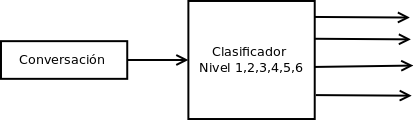
\includegraphics[scale=.5]{images/arquitecturaprotipo4}
\caption{Arquitectura prototipo 4}
\label{fig:arquitecturaNivel4}
\end{center}
\end{figure} 

\subsection{Dise\~no de la red neuronal}
La arquitectura que tendr\'a la red neuronal est\'a presentado en la figura \ref{fig:redNeuronal} donde la capa de entrada represantan los vectores de los niveles descritos anteriormente, la capa oculta est\'a constituida por 7 neuronas y la capa de salida por 4.

\begin{figure}
\begin{center}
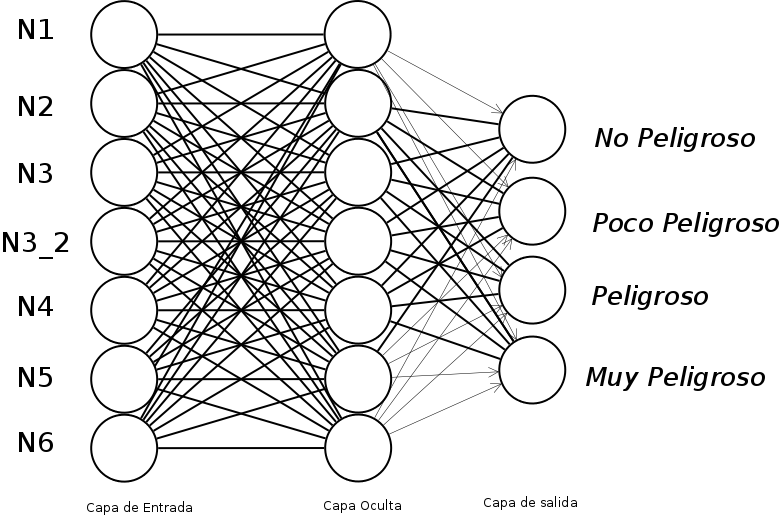
\includegraphics[scale=.3]{images/redneuronal}
\caption{Arquitectura de la Red Neuronal del prototipo 4}
\label{fig:redNeuronal}
\end{center}
\end{figure}

Dicha red fue entrenada con el algorimo de aprendizaje Backpropagation.

\section{Pruebas} 

%La figurura \ref{fig:mconfucion} muestra la matriz de confusi\'on donde se muestra una precisi\'on del 98.9\%.

%\begin{figure}[h]
%\begin{center}
%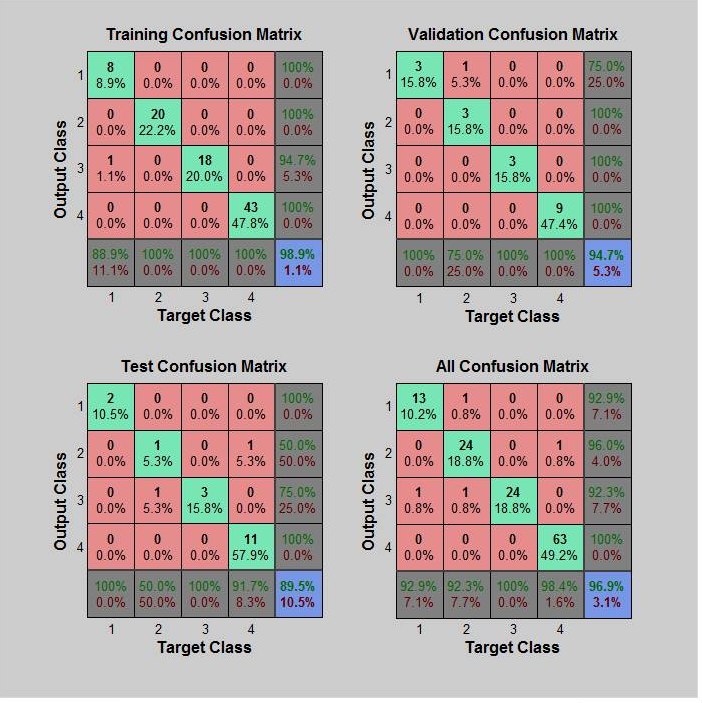
\includegraphics[scale=.5]{images/mcofucion}
%\caption{Matriz de confusi\'on del clasificador}
%\label{fig:mconfucion}
%\end{center}
%\end{figure}
La tabla \ref{tab:tablaresultadosconjuntoentrenamientopeligroso} muestra los resultados de las conversaciones con las que entrenamos el algoritmo de regresi\'on log\'istica en el prototipo anterior ahora sometidos a la entrada de la red neuronal. La diferenci\'ia entre un resultado y otro es que las conversaciones que con anterioridad hab\'ian sido marcadas como no peligrosas, ahora la red neuronal la ha clasificado como Peligrosas y Poco Peligrosas de acuerdo a su vector de frecuencias de frases de los dem\'as niveles. 
\begin{table}[h]
\small
\begin{tabular}{|c|c|c|c|c|c|c|c|c|c|}
\hline
Conversacion & N1 & N2 & N3 & N3\_2 & N4 & N5 & N6 & Espectativa de Resultado & Resultado \\

peligrosas/10.txt
& 0
& 2
& 5
& 3
& 0
& 1
& 0
& Muy Peligrosa
& Muy Peligrosa \\
peligrosas/11.txt
&  0
& 2
& 2
& 0
& 0
& 1
& 0
& Muy Peligrosa
& Muy Peligrosa \\

peligrosas/12.txt
&  0
& 2
& 0
& 0
& 0
& 1
& 1
& Muy Peligrosa
& Muy Peligrosa \\
peligrosas/13.txt 
&  0
& 2
& 2
& 0
& 0
& 1
& 1
& Muy Peligrosa
& Muy Peligrosa \\
peligrosas/14.txt 
&  0
& 4
& 0
& 0
& 0
& 1
& 1
& Muy Peligrosa
& Muy Peligrosa \\
peligrosas/15.txt
&  0
& 2
& 0
& 0
& 0
& 1
& 1
& Muy Peligrosa
& Muy Peligrosa \\
peligrosas/16.txt
&  0
& 6
& 4
& 2
& 0
& 1
& 0
& Muy Peligrosa
& Muy Peligrosa \\
peligrosas/17.txt
&  0
& 0
& 0
& 0
& 0
& 1
& 0
& Muy Peligrosa
& Muy Peligrosa \\
peligrosas/18.txt
&  2
& 6
& 6
& 4
& 0
& 0
& 1
& Peligrosa
& Peligrosa  \\
peligrosas/19.txt
&  0
& 11
& 3
& 1
& 0
& 1
& 3
& Muy Peligrosa
& Muy Peligrosa \\
peligrosas/1tx.txt
&  2
& 10
& 0
& 0
& 1
& 1
& 3
& Muy Peligrosa
& Muy Peligrosa \\
peligrosas/20.txt
&  1
& 0
& 0
& 0
& 0
& 1
& 2
& Muy Peligrosa
& Muy Peligrosa \\
peligrosas/21.txt
&  0
& 5
& 0
& 0
& 0
& 1
& 0
& Muy Peligrosa
& Muy Peligrosa \\
peligrosas/22.txt
&  0
& 1
& 1
& 0
& 0
& 1
& 0
& Muy Peligrosa
& Muy Peligrosa \\
peligrosas/23.txt
&  1
& 4
& 1
& 0
& 0
& 1
& 0
& Muy Peligrosa
& Muy Peligrosa \\
peligrosas/24.txt
&  1
& 0
& 0
& 0
& 1
& 1
& 0
& Muy Peligrosa
& Muy Peligrosa \\
peligrosas/25.txt
&  4
& 7
& 5
& 3
& 0
& 1
& 0
& Muy Peligrosa
& Muy Peligrosa \\
peligrosas/26.txt
&  0
& 1
& 0
& 0
& 0
& 1
& 0
& Muy Peligrosa
& Muy Peligrosa \\
peligrosas/27.txt
&  0
& 0
& 0
& 0
& 0
& 1
& 0
& Muy Peligrosa
& Muy Peligrosa \\
peligrosas/28.txt
&  0
& 1
& 3
& 1
& 0
& 1
& 0
& Muy Peligrosa
& Muy Peligrosa \\
peligrosas/29.txt
&  0
& 0
& 2
& 0
& 0
& 1
& 2
& Muy Peligrosa
& Muy Peligrosa \\
peligrosas/2.txt
&  0
& 5
& 2
& 0
& 0
& 1
& 2
& Muy Peligrosa
& Muy Peligrosa \\
peligrosas/30.txt
&  1
& 6
& 4
& 2
& 0
& 1
& 0
& Muy Peligrosa
& Muy Peligrosa \\
peligrosas/31.txt
&  0
& 1
& 1
& 0
& 1
& 1
& 0
& Muy Peligrosa
& Muy Peligrosa \\
peligrosas/32.txt
&  0
& 0
& 0
& 0
& 0
& 1
& 0
& Muy Peligrosa
& Muy Peligrosa \\
peligrosas/33.txt
&  0
& 3
& 0
& 0
& 0
& 1
& 1
& Muy Peligrosa
& Muy Peligrosa \\
peligrosas/34.txt
&  0
& 4
& 0
& 0
& 0
& 1
& 0
& Muy Peligrosa
& Muy Peligrosa \\
peligrosas/35.txt
&  0
& 0
& 6
& 4
& 0
& 1
& 0
& Muy Peligrosa
& Muy Peligrosa \\
peligrosas/36.txt
&  0
& 9
& 8
& 6
& 0
& 1
& 0
& Muy Peligrosa
& Muy Peligrosa \\
peligrosas/37.txt
&  0
& 3
& 0
& 0
& 0
& 1
& 1
& Muy Peligrosa
& Muy Peligrosa \\
peligrosas/38.txt
&  1
& 2
& 8
& 6
& 0
& 1
& 1
& Muy Peligrosa
& Muy Peligrosa \\
peligrosas/39.txt
&  0
& 1
& 1
& 0
& 0
& 1
& 0
& Muy Peligrosa
& Muy Peligrosa \\
peligrosas/3.txt
&  0
& 1
& 0
& 0
& 0
& 1
& 0
& Muy Peligrosa
& Muy Peligrosa \\
peligrosas/40.txt
&  0
& 5
& 1
& 0
& 0
& 1
& 1
& Muy Peligrosa
& Muy Peligrosa \\
%peligrosas/4.txt
%&  1
%& 3
%& 1
%& 0
%& 0
%& 0
%& 1
%& No Peligrosa
%& No Peligrosa \\
peligrosas/5.txt
&  0
& 4
& 0
& 0
& 0
& 1
& 0
& Muy Peligrosa
& Muy Peligrosa \\
peligrosas/6.txt
&  1
& 4
& 3
& 1
& 0
& 1
& 0
& Muy Peligrosa
& Muy Peligrosa \\
peligrosas/7.txt
&  0
& 4
& 1
& 0
& 2
& 0
& 0
& Poco Peligrosa
& Poco Peligrosa \\
peligrosas/8.txt
&  3
& 13
& 1
& 0
& 0
& 1
& 0
& Muy Peligrosa
& Muy Peligrosa \\
peligrosas/9.txt
&  0
& 6
& 3
& 1
& 0
& 1
& 0
& Muy Peligrosa
& Muy Peligrosa \\
peligrosas/cp1.txt
&  1
& 6
& 7
& 5
& 0
& 1
& 0
& Muy Peligrosa
& Muy Peligrosa \\
peligrosas/cp2.txt
&  2
& 22
& 10
& 8
& 0
& 1
& 1
& Muy Peligrosa
& Muy Peligrosa \\
peligrosas/cp3.txt
&  6
& 7
& 14
& 12
& 0
& 1
& 2
& Muy Peligrosa
& Muy Peligrosa \\
peligrosas/cp4.txt
&  1
& 2
& 2
& 0
& 0
& 1
& 1
& Muy Peligrosa
& Muy Peligrosa \\
peligrosas/cp6.txt
&  3
& 5
& 5
& 3
& 0
& 1
& 3
& Muy Peligrosa
& Muy Peligrosa \\
peligrosas/cp7.txt
&  0
& 11
& 5
& 3
& 0
& 1
& 2
& Muy Peligrosa
& Muy Peligrosa \\
\hline
\end{tabular}
\label{tab:tablaresultadosconjuntoentrenamientopeligroso}
\caption{Resultado del an\'alisis del conjunto de conversaciones peligrosas de entrenamiento}
\end{table}

La tabla \ref{tab:tablaresultadosconjuntoentrenamientonopeligroso} Muestra los resultados de las conversaciones no peligrosas del conjunto de entrenamiento del algoritmo de regresi\'on log\'istica ahora como entrada a al red neuronal. La diferencia entre ambos resultados es que una conversaci\'on ha sido marcada como Poco Peligrosa debido a que el tipo de frases que tiene hacen que esa conversaci\'on pudiera tener tendencias a convertirse en una conversaci\'on de riesgo.
\begin{table}[h]
\small
\begin{tabular}{|c|c|c|c|c|c|c|c|c|c|}
\hline
Conversacion & N1 & N2 & N3 & N3\_2 & N4 & N5 & N6 & Espectativa de Resultado & Resultado \\

np/cnp10.txt
& 0
& 2
& 0
& 0
& 0
& 0
& 0
& No Peligrosa
& No Peligrosa \\
np/cnp11.txt
& 0
& 2
& 0
& 0
& 0
& 0
& 0
& No Peligrosa
& No Peligrosa \\
np/cnp13.txt
& 0
& 0
& 0
& 0
& 0
& 0
& 0
& No Peligrosa
& No Peligrosa \\
np/cnp14.txt
& 0
& 2
& 0
& 0
& 0
& 0
& 0
& No Peligrosa
& No Peligrosa \\ 
np/cnp16.txt
& 0
& 3
& 0
& 0
& 0
& 0
& 1
& Poco Peligrosa
& Poco Peligrosa \\
np/cnp17.txt
& 1
& 1
& 0
& 0
& 0
& 0
& 0
& No Peligrosa
& No Peligrosa \\
np/cnp18.txt
& 2
& 4
& 0
& 0
& 0
& 0
& 0
& No Peligrosa
& No Peligrosa\\
np/cnp19.txt
& 0
& 3
& 0
& 0
& 0
& 0
& 0
& No Peligrosa
& No Peligrosa \\
np/cnp1.txt
& 0
& 4
& 1
& 0
& 0
& 0
& 3
& No Peligrosa
& No Peligrosa \\
np/cnp20.txt
& 0
& 0
& 0
& 0
& 0
& 0
& 0
& No Peligrosa
& No Peligrosa \\
np/cnp15.txt
& 0
& 1
& 0
& 0
& 0
& 0
& 0
& No Peligrosa
& No Peligrosa \\
np/cnp2.txt
& 0
& 1
& 2
& 0
& 0
& 0
& 1
& No Peligrosa
& No Peligrosa \\
np/cnp3.txt
& 0
& 1
& 0
& 0
& 0
& 0
& 0
& No Peligrosa
& No Peligrosa \\
np/cnp4.txt
& 0
& 1
& 0
& 0
& 0
& 0
& 0
& No Peligrosa
& No Peligrosa \\
np/cnp5.txt
& 0
& 2
& 0
& 0
& 0
& 0
& 0
& No Peligrosa
& No Peligrosa \\
np/cnp6.txt
& 0
& 1
& 2
& 0
& 0
& 0
& 0
& No Peligrosa
& No Peligrosa \\
np/cnp7.txt
& 0
& 1
& 1
& 0
& 0
& 0
& 0
& No Peligrosa
& No Peligrosa \\
np/cnp9.txt
& 1
& 2
& 0
& 0
& 0
& 0
& 0
& No Peligrosa
& No Peligrosa \\
np/cnp8.txt
& 1
& 0
& 0
& 0
& 0
& 0
& 0
& No Peligrosa
& No Peligrosa \\
np/cnp12.txt
& 0
& 0
& 0
& 0
& 0
& 0
& 0
& No Peligrosa
& No Peligrosa \\
\hline
\end{tabular}
\label{tab:tablaresultadosconjuntoentrenamientonopeligroso}
\caption{Resultado del an\'alisis del conjunto de conversaciones peligrosas de entrenamiento}
\end{table}

La tabla \ref{tab:redpruebas} muestra los resultados del validaci\'on sumando los resultados de las tablas \ref{tab:tablaresultadosconjuntopruebapeligroso} y \ref{tab:tablaresultadosconjuntopruebanopeligroso} aquí se muestra que para los conjuntos de prueba se ha obtenido un 100\% para los valores predichos con relaci\'on a los esperados.
\begin{table}[h]
\begin{center}
\begin{tabular}{c|c|c|c|c|c|c|}
\multicolumn{5}{c}{Predicci\'on} \\
\cline{2-7}
& &  Muy Peligrosa & Peligrosas & Poco Peligrosa & No peligrosa &  Precisi\'on \\
\cline{2-7}
\multirow{2}{*}{Actual} & Muy Peligrosa & 41 & 0 & 0 & 0 & 100\% \\
\cline{2-7}
& Conversaci\'on Peligrosa & 0 & 1 &  0 & 0 & 100\% \\
\cline{2-7}
& Conversaci\'on Poco Peligrosa & 0 & 0 &  2 & 0 & 0\% \\
\cline{2-7}
& Conversaci\'on No Peligrosa & 0 & 0 &  0 & 19 & 100\% \\
\cline{2-7}


\end{tabular}
\caption{Tabla de validaci\'on del conjunto de entrenamiento en la red neuronal}
\label{tab:redpruebas}
\end{center}
\end{table}

\begin{table}[h]
\begin{center}
\begin{tabular}{c|cc|c|c|}
& Precision & Recall & Average & $F_1 Score$ \\
\hline
Conjunto de Entrenamiento & 1 & 1 & 1 &  1 \\ 

\end{tabular}

\label{tab:valores}
\caption{Tabla de Valores de Promedio y $F_1$ para la red neuronal del conjunto de entrenamiento}
\end{center}
\end{table}


La tabla \ref{tab:tablaresultadosconjuntopruebapeligroso} muestra los resultados de las conversaciones de prueba que hemos marcado como peligrosas. La columna de espectativa es el resultado que se espera obtener , mientras que la de resultado es el obtenido que se obtuvo a la salida del clasificador.

\begin{table}[h]
\begin{tabular}{|c|c|c|c|c|c|c|c|c|c|}
\hline
Conversacion & N1 & N2 & N3 & N3\_2 & N4 & N5 & N6 & Espectativa de Resultado & Resultado \\

\hline
pr10.txt &  0 & 3 & 0 & 0 & 0 & 1 & 1 & Muy Peligrosa & Muy Peligrosa \\
\hline
pr11.txt &  0 & 4 & 0 & 0 & 0 & 1 & 0 & Muy Peligrosa & Muy Peligrosa \\
\hline
pr12.txt &  0 & 0 & 6 & 4 & 0 & 1 & 0 & Muy Peligrosa & Muy Peligrosa \\
\hline
pr15.txt &  0 & 13 & 4 & 2 & 1 & 0 & 0 & Peligrosa & Peligrosa \\
\hline
pr16.txt &  1& 4 & 1 & 0 & 0 & 1 & 0 & Muy Peligrosa & Muy Peligrosa \\
\hline
pr17.txt &  1 & 0 & 0 & 0 & 1 & 1 & 0 & Muy Peligrosa & Muy Peligrosa \\
\hline
pr18.txt &  4 & 7 & 5 & 3 & 0 & 1 & 0 & Muy Peligrosa & Muy Peligrosa \\
\hline
pr1.txt &  2 & 10 & 0 & 0 & 1 & 1 & 3 & Muy Peligrosa & Muy Peligrosa \\
\hline
pr21.txt &  1 & 1 & 0 & 0 & 0 & 1 & 0 & Muy Peligrosa & Muy Peligrosa \\
\hline
pr22.txt &  0 & 4 & 0 & 0 & 0 & 1 & 0& Muy Peligrosa & Muy Peligrosa \\
\hline
pr4.txt &  0 & 1 & 0 & 0 & 0 & 1 & 0 & Muy Peligrosa & Muy Peligrosa \\
\hline
pr5.txt &  0 & 0 & 0 & 0 & 0 & 1 & 0 & Muy Peligrosa & Muy Peligrosa \\
\hline
pr6.txt & 0 & 1 & 3 & 1 & 0 & 1 & 0 & Muy Peligrosa & Muy Peligrosa \\
\hline
pr7.txt &  1 & 6 & 4 & 2 & 0 & 1 & 0 & Muy Peligrosa & Muy Peligrosa \\
\hline
pr8.txt &  0 & 1 & 1 & 0 & 1 & 1 & 0 & Muy Peligrosa & Muy Peligrosa \\
\hline
pr9.txt &  0 & 0 & 0 & 0 & 0 & 1 & 0 & Muy Peligrosa & Muy Peligrosa \\
\hline
prueba1.txt &  0 & 0 & 0 & 0 & 0 & 0 & 0 & No Peligrosa & No Peligrosa \\
\hline
prueba2.txt &  0 & 4 & 0 & 0 & 0 & 1 & 0 & Muy Peligrosa & Muy Peligrosa \\
\hline
prueba3.txt  &  0 & 3& 6 & 4 & 0 & 1 & 0 & Muy Peligrosa & Muy Peligrosa \\
\hline
prueba4.txt  &  0 & 5 & 1 & 0 & 0 & 1 & 0 & Muy Peligrosa & Muy Peligrosa \\
\hline
prueba5.txt &  0 & 1 & 0 & 0 & 0 & 0 & 0 & No Peligrosa  & No Peligrosa \\
\hline
prueba6.txt &  1 & 3 & 0 & 0 & 0 & 0& 0 & No Peligrosa & No Peligrosa \\
\hline
prueba7.txt &  0 & 13 & 2 & 0 & 0 & 1 & 0 & Muy Peligrosa & Muy Peligrosa \\
\hline
prueba8.txt &  0 & 1 & 2 & 0 & 0 & 1 & 3 & Muy Peligrosa & Muy Peligrosa \\ 
\hline
prueba9.txt &  0 & 4 & 1 & 0 & 0 & 1 & 3 & Muy Peligrosa & Muy Peligrosa \\
\hline

\end{tabular}
\label{tab:tablaresultadosconjuntopruebapeligroso}
\caption{Resultado del an\'alisis del conjunto de conversaciones peligrosas}
\end{table}
La tabla \ref{tab:tablaresultadosconjuntopruebapeligroso} muestra los resultados de las conversaciones de prueba no peligrosas. La columna de espectativa es el resultado que se espera obtener , mientras que la de resultado es el obtenido que se obtuvo a la salida del clasificador.

\begin{table}
\begin{tabular}{|c|c|c|c|c|c|c|c|c|c|}
\hline
Conversacion & N1 & N2 & N3 & N3\_2 & N4 & N5 & N6 & Espectativa de Resultado & Resultado \\

\hline
npr10.txt &  1 & 2 & 0 & 0 & 0 & 0 & 1 & No peligrosa & No peligrosa \\
\hline
npr11.txt &  0 & 1 & 0 & 0 & 0 & 0 & 0 & No peligrosa & No peligrosa \\
\hline
npr12.txt &  0 & 0 & 6 & 0 & 0 & 0 & 0 & No peligrosa & No peligrosa \\
\hline
npr15.txt &  0 & 0 & 4 & 0 & 0 & 0 & 0 & No peligrosa & No peligrosa \\
\hline
npr16.txt &  1 & 4 & 1 & 0 & 0 & 0 & 0 & No peligrosa & No peligrosa \\
\hline
npr17.txt &  1 & 0 & 0 & 0 & 1 & 0 & 0 & No peligrosa & No peligrosa \\
\hline
npr18.txt &  4 & 7 & 5 & 0 & 0 & 0 & 0 & No peligrosa & No peligrosa \\
\hline
npr1.txt &  2 & 1 & 0 & 0 & 1 & 0 & 3 & No peligrosa & No peligrosa \\
\hline
npr21.txt &  1 & 1 & 0 & 0 & 0 & 0 & 0 & No peligrosa & No peligrosa \\
\hline
npr22.txt &  0 & 1 & 0 & 0 & 0 & 0 & 0& No peligrosa & No peligrosa \\
\hline
npr4.txt &  0 & 1 & 0 & 0 & 0 & 0 & 0 & No peligrosa & No peligrosa \\
\hline
npr5.txt &  0 & 0 & 0 & 0 & 0 & 0 & 0 & No peligrosa & No peligrosa \\
\hline
npr6.txt & 0 & 1 & 3 & 0 & 0 & 0 & 0 & No peligrosa & No peligrosa \\
\hline
npr7.txt &  1 & 2 & 4 & 0 & 0 & 0 & 0 & No peligrosa & No peligrosa \\
\hline
npr8.txt &  0 & 1 & 1 & 0 & 1 & 0 & 0 & No peligrosa & No peligrosa \\
\hline
npr9.txt &  0 & 0 & 0 & 0 & 0 & 0 & 0 & No peligrosa & No peligrosa \\
\hline
nprueba1.txt &  0 & 0 & 0 & 0 & 0 & 0 & 0 & No Peligrosa & No Peligrosa \\
\hline
nprueba2.txt &  0 & 4 & 0 & 0 & 0 & 0 & 0 & No peligrosa & No peligrosa \\
\hline
nprueba3.txt  &  0 & 3& 0 & 4 & 0 & 0 & 0 & No peligrosa & No peligrosa \\
\hline
nprueba4.txt  &  0 & 5 & 1 & 0 & 0 & 1 & 0 & Muy peligrosa & Muy peligrosa \\
\hline
nprueba5.txt &  0 & 1 & 0 & 0 & 0 & 0 & 0 & Muy peligrosa  & Muy peligrosa \\
\hline
nprueba6.txt &  1 & 3 & 0 & 0 & 0 & 1 & 0 & No Peligrosa & No Peligrosa \\
\hline
nprueba7.txt &  0 & 0 & 2 & 0 & 0 & 0 & 0 & No peligrosa & No peligrosa \\
\hline
nprueba8.txt &  0 & 1 & 2 & 0 & 0 & 0 & 3 & No peligrosa & No peligrosa \\ 
\hline
nprueba9.txt &  0 & 2 & 1 & 0 & 0 & 0 & 3 & No peligrosa & No peligrosa \\
\hline

\end{tabular}
\label{tab:tablaresultadosconjuntopruebanopeligroso}
\caption{Resultado del an\'alisis del conjunto de conversaciones no peligrosas}
\end{table}

La tabla \ref{tab:redpruebas} muestra los resultados del validaci\'on sumando los resultados de las tablas \ref{tab:tablaresultadosconjuntopruebapeligroso} y \ref{tab:tablaresultadosconjuntopruebanopeligroso} aquí se muestra que para los conjuntos de prueba se ha obtenido un 100\% para los valores predichos con relaci\'on a los esperados.
\begin{table}[h]
\begin{center}
\begin{tabular}{c|c|c|c|c|c|c|}
\multicolumn{5}{c}{Predicci\'on} \\
\cline{2-7}
& &  Muy Peligrosa & Peligrosas & Poco Peligrosa & No peligrosa &  Precisi\'on \\
\cline{2-7}
\multirow{2}{*}{Actual} & Muy Peligrosa & 23 & 0 & 0 & 0 & 100\% \\
\cline{2-7}
& Conversaci\'on Peligrosa & 0 & 1 &  0 & 0 & 100\% \\
\cline{2-7}
& Conversaci\'on Poco Peligrosa & 0 & 0 &  0 & 0 & 0\% \\
\cline{2-7}
& Conversaci\'on No Peligrosa & 0 & 0 &  0 & 26 & 100\% \\
\cline{2-7}


\end{tabular}
\caption{Tabla de validaci\'on del conjunto de pruebas en la red neuronal}
\label{tab:redpruebas}
\end{center}
\end{table}

\begin{table}[h]
\begin{center}
\begin{tabular}{c|cc|c|c|}
& Precision & Recall & Average & $F_1 Score$ \\
\hline
Conjunto de Entrenamiento & 1 & 1 & 1 &  1 \\ 

\end{tabular}

\label{tab:valores}
\caption{Tabla de Valores de Promedio y $F_1$ para la red neuronal del conjunto de pruebas}
\end{center}
\end{table}